\section{SOA}
\subsection{Primeros conceptos}

Los conceptos base del diseño de software deben ser expuestos para tener una mayor claridad en los temas siguientes. A continuación se expresan los conceptos base:

\begin{itemize}
  \item Características de diseño: Son aquellos atributos que cumple un diseño y que pueden ser medidos

  \item Principio de diseño: Es una guía o regla para solucionar un problema de acuerdo a las prácticas aceptadas por la comunidad de ingeniería de software.

  \item Paradigma de diseño: Es el compendio de principios de diseño que tienen un enfoque global común.

  \item Patrones de diseño: Son formas de resolver un problema de diseño que es repetitivo. Viene dado por 3 restricciones presentadas en el diseño de software:
  \begin{itemize}
    \item Restricciones impuestas por la tecnología existente
	  \item Restricciones impuestas por las tecnologías usadas por sistemas transversales
	  \item Restricciones de prioridades de proyectos
  \end{itemize}
  El patrón de diseño describe el problema y da la solución a modo de plantilla.

  \item Lenguajes de patrones de diseño: Es la configuración ordenada de patrones en un diseño lógico. La comunicación entre cada patrón se hace a través de dicho lenguaje.

  \item Estandares de diseño: En orden de ir acorde a las metas, prioridades, recursos y ambiente de la organización en la que se haga el diseño lógico de la solución, un estandar de diseño define convenciones para cada elemento utilizado en el diseño de acuerdo a las características de diseño definidas.

  \item Buenas prácticas: Es una técnica o acercamiento para resolver o prevenir problemas presentados en el desarrollo del diseño lógico de la solución de software. pg 34
\end{itemize}

La figura \ref{fig:uno} presenta un acercamiento a cómo se desarrollan los principios de diseño con los demás conceptos nombrados.

\begin{figure}[!htb]
  \begin{center}
    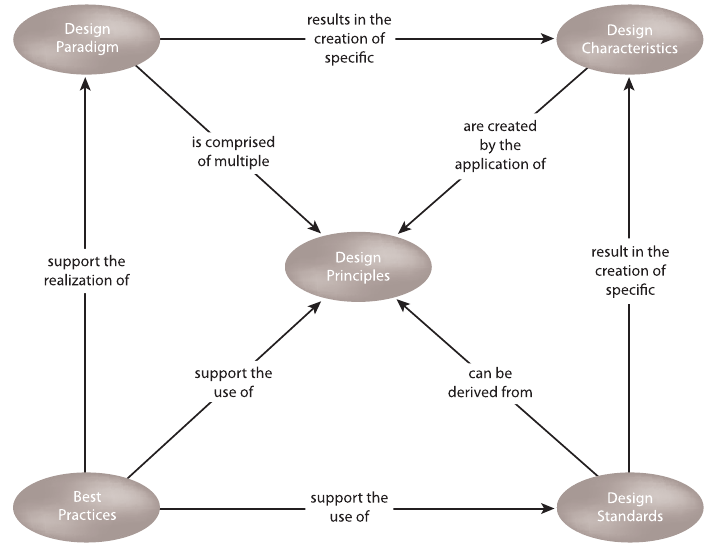
\includegraphics[width=11cm]{./imagenes/1.png}
    \caption{Ejemplo de uso del enlace exclusivo}
    \label{fig:uno}
  \end{center}
\end{figure}

La figura \ref{fig:dos} presenta cómo extiende o soporta un patrón de diseño el diseño lógico de la solución de software.

\begin{figure}[!htb]
  \begin{center}
    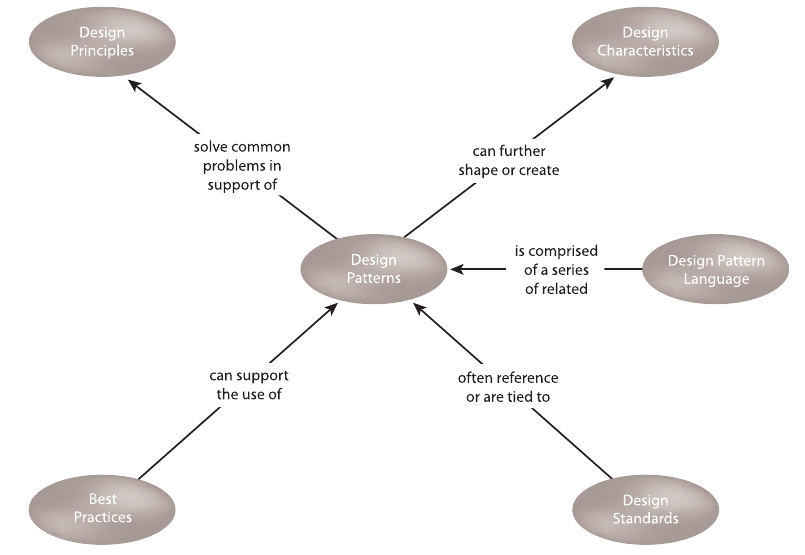
\includegraphics[width=11cm]{./imagenes/2.png}
    \caption{Ejemplo de uso del enlace exclusivo}
    \label{fig:dos}
  \end{center}
\end{figure}

La figura \ref{fig:tres} presenta los componentes que hacen que el diseño lógico de la solución sea acorde al paradigma escogido.

\begin{figure}[!htb]
  \begin{center}
    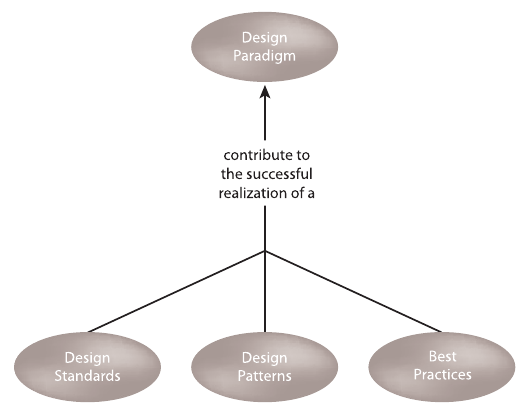
\includegraphics[width=11cm]{./imagenes/3.png}
    \caption{Ejemplo de uso del enlace exclusivo}
    \label{fig:tres}
  \end{center}
\end{figure}

\subsection{Computación orientada a servicios}

La computación orientada a servicios nace de la necesidad de desarrollar software sobre tecnologías distribuidas. Este tipo de computación tiene como finalidad la construcción de inventarios de servicios. La computación orientada a servicios está compuesta por la interacción de la orientación a servicios y la arquitectura orientada a servicios, formando patrones de diseño propios y estándares en cumplimiento de las características de diseño propias de la computación distribuida. Algunos de los conceptos clave llevados en la computación orientada a servicios son:

\begin{itemize}
  \item Arquitectura Orientada a Servicios (SOA - Service Oriented Architecture): Comprende el compendio de tecnologías, APIs, infraestructura y repositorios enmarcados en
el paradigma orientado a servicios y cuyo objetivo principal es el de trabajar sobre el "servicio" como el elemento más importante.

  \item Orientación a servicios: Es el paradigma manejado en la computación orientada a servicios en donde se acepta como unidad mínima y más importante el "servicio"

  \item Servicio: Es un software independiente físicamente el cual tiene asignado un contexto de funcionalidades y que puede ser utilizado por otros servicios por medio
del contrato del servicio (descripción del servicio en cuanto a funcionalidades, entradas requeridas y salidas). De acuerdo a su nivel de reuso, los servicios se dividen en 3 tipos y son:
  \item Servicios entidad: Modela los servicios que se deben ofrecer respecto de las entidades del negocio (ej. empleados y clientes). Tienen un nivel de reuso alto y están centrados en el negocio.
  \item Servicios tarea: Modela los servicios que deben cumplir tareas específicas del negocio (ej. generación de cortes de final de año). Tienen un nivel de reuso bajo. Estos servicios trabajan directamente con 1 o varios servicios entidad. Estos servicios están centrados en el negocio.
  \item Servicios utilidad: Modela servicios que no están centrados en el negocio. Son los servicios con mayor reuso.
La diferenciación entre tipos de servicio da lugar a la estructura en capas mostrada en la figura \ref{fig:cinco}

  \item Composición de servicios: Es la agregación de servicios de manera ordenada.

  \item Inventario de servicios: Es la agrupación de varios servicios según un criterio definido por la organización. Cada inventario de servicios tiene su propio estándar
de diseño e, inclusive, su propia configuración arquitectónica. El desarrollo de los inventarios de servicio es hecho a modo top-down, con la construcción de blueprints (planos).
\end{itemize}

\begin{figure}[!htb]
  \begin{center}
    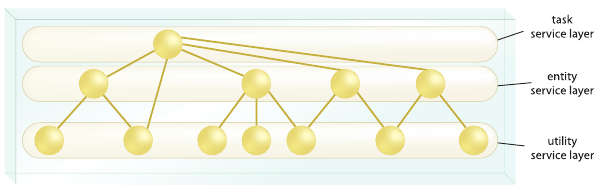
\includegraphics[width=11cm]{./imagenes/5.png}
    \caption{Ejemplo de uso del enlace exclusivo}
    \label{fig:cinco}
  \end{center}
\end{figure}

En la figura \ref{fig:cuatro} se muestra la interacción de los conceptos clave en la computación orientada a servicios.

\begin{figure}[!htb]
  \begin{center}
    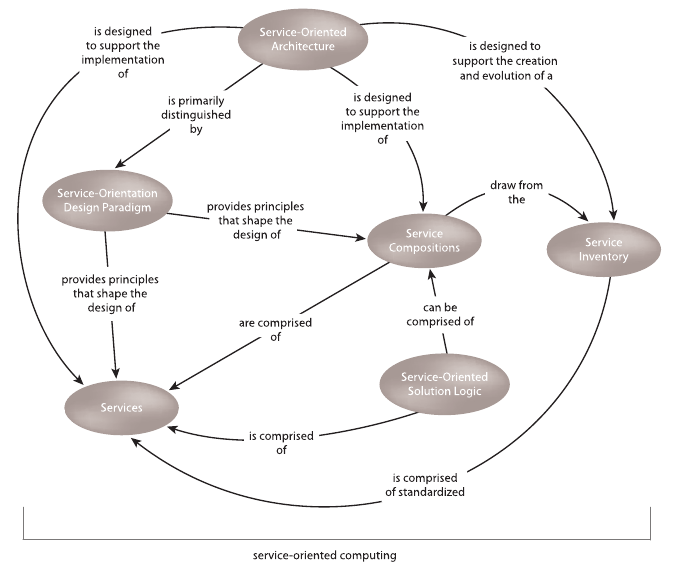
\includegraphics[width=11cm]{./imagenes/4.png}
    \caption{Ejemplo de uso del enlace exclusivo}
    \label{fig:cuatro}
  \end{center}
\end{figure}
